
%%%%%%%%%%%%%%%%%%%%%%% file typeinst.tex %%%%%%%%%%%%%%%%%%%%%%%%%
%
% This is the LaTeX source for the instructions to authors using
% the LaTeX document class 'llncs.cls' for contributions to
% the Lecture Notes in Computer Sciences series.
% http://www.springer.com/lncs       Springer Heidelberg 2006/05/04
%
% It may be used as a template for your own input - copy it
% to a new file with a new name and use it as the basis
% for your article.
%
% NB: the document class 'llncs' has its own and detailed documentation, see
% ftp://ftp.springer.de/data/pubftp/pub/tex/latex/llncs/latex2e/llncsdoc.pdf
%
%%%%%%%%%%%%%%%%%%%%%%%%%%%%%%%%%%%%%%%%%%%%%%%%%%%%%%%%%%%%%%%%%%%


\documentclass[runningheads,a4paper]{llncs}

\usepackage{amssymb}
\setcounter{tocdepth}{3}
\usepackage{graphicx}
\usepackage{float}
\usepackage{subfigure}

\usepackage{pgfplots}
\usepackage{url}
\usepackage{enumitem}
\usepackage[linesnumbered,ruled]{algorithm2e}
\usepackage[export]{adjustbox}
\usepackage{xspace}
\usepackage{breqn}

\newcommand{\sgg}{{\sc Smart GeoGuide}}
\newcommand{\geoguide}{{\sc GeoGuide}}

\usepackage{url}


\urldef{\mailsb}\path|placido.neto@ifrn.edu.br|   
\urldef{\mailsc}\path|Behrooz.Omidvar-Tehrani@univ-grenoble-alpes.fr|    
\urldef{\mailsd}\path|{tiago.oliveira, bento.francisco, freire.pontes}@academico.ifrn.edu.br|
\newcommand{\keywords}[1]{\par\addvspace\baselineskip
\noindent\keywordname\enspace\ignorespaces#1}

\begin{document}

\mainmatter  % start of an individual contribution

% first the title is needed
\title{\sgg: an approach for highlighting points in spatial data}

% a short form should be given in case it is too long for the running head
\titlerunning{\sgg: an smart approach for highlighting points in spatial data}

% the name(s) of the author(s) follow(s) next
%
% NB: Chinese authors should write their first names(s) in front of
% their surnames. This ensures that the names appear correctly in
% the running heads and the author index.
%
\author{Pl\'acido A. Souza Neto \and  Behrooz Omidvar-Tehrani \and Tiago Oliveira Lisboa \and \\
Francisco B. Silva Junior \and Felipe F. Pontes }
%
\authorrunning{Souza Neto, Pl\'acido A. \textit{et al.}}
% (feature abused for this document to repeat the title also on left hand pages)

% the affiliations are given next; don't give your e-mail address
% unless you accept that it will be published
\institute{Federal Institute of Rio Grande do Norte (Brazil)\\
\mailsb\\
\mailsd\\
University of Grenoble Alpes (France)\\ 
\mailsc\\
}



%
% NB: a more complex sample for affiliations and the mapping to the
% corresponding authors can be found in the file "llncs.dem"
% (search for the string "\mainmatter" where a contribution starts).
% "llncs.dem" accompanies the document class "llncs.cls".
%

\toctitle{Lecture Notes in Computer Science}
\tocauthor{Authors' Instructions}
\maketitle


\begin{abstract}


In this paper we present a solution to capture region preferences from implicit feedbacks. Given a point from a spatial dataset, a set of regions captured from gaze and mouse tracking, the set of region intersections, the \sgg\ captures the implicit feedback of analysts and exploits it to highlight potentially interesting options. The analysis consider the concept of relevance and diversity of a given point with the others in the same data set, from the regions tracked during the analysis.  To tackle this challenge, we extend \geoguide \cite{Omidvar:2017} approach by using ST-DBSCAN\cite{Birant:2007} algorithm to map the region preferences from implicit tracking over time. We capture, analyse, generate and save region preferences in order to highlight informations, from any spatial dataset that can be useful to the analyst. So, this work aims to answers questions about interactivity and guidance in spatial solutions. We evaluate the efficiency of the proposed approach experimentally considering spatial datasets.

\keywords{\sgg, ST-DBSCAN, mouse-tracking, implicit preferences, regions}
\end{abstract}


\section{Introduction}

During spatial data analysis, it is often the case that analysts look at some regions of interest. For instance in Example~\ref{ex:benicio},  \textit{Ben\'icio} looks for a good appartment in Paris. While he is focusing on home-stays close to the Eiffel tower, he also looks at farther locations with easy train access, close to \textit{boulangeries} and good restaurants. However, he never clicks on those points. 

\begin{example}
\label{ex:benicio}
\textit{Ben\'icio} is planning to live a season in Paris. He decides to rent a home-stay from Airbnb website\footnote{\it http://www.airbnb.com}. As he already know the city, because he has already visited several times before decide to spend a season for study, he is open to any type of lodging, considering some regions of his preferences. He wants to explore his options very carefully. He queries all available locations in Paris with a fair price, although he prefers to live in a more central area of the city, to take better advantage of what Paris can offer. His query results in 3000 locations. As he has no other preferences, an exhaustive investigation needs scanning each location independently which is nearly infeasible. In case he wants to focus on a smaller set of options, it is not clear which subset he needs to look at. While he is looking at primary locations in the list, he shows interest in having ``balcony'' as amenity and being close to Eiffel tower. An ideal system can capture this feedback through mouse-tracking, for instance, in order to short-list a small subset of remaining locations that \textit{Ben\'icio} should consider as high priority based on the regions  which he searched through the mouse movement made on the map of Paris. 
\end{example}

In spatialtemporal data analysis, it is often the case that analysts look at some regions of interest but forget to provide an explicit feedback. To capture user preferences is necessary go beyond filling in attributes and data provided by the user. It is important to understand the user behaviour while using the application to infer about his possible preferences. \cite{Robertson2007}  affirms that temporal change in spatial patterns are increasingly common in geographical analysis. This work explore an approach to the spatialtemporal analysis of polygons that are spatially distinct and experience discrete changes though time. It presents challenges considering changes of regions (polygons) during the time. Works like \cite{Ester:1996} and  \cite{Birant:2007} present solutions for clustering spatialtemporal data. These solutions are relevant to define regions by each cluster that contains important informations for the user. 

It is shown in \cite{Arapakis:2014} that mouse gestures have a strong correlation with ``user engagement''. Intuitively, a point receives a positive feedback if the cursor moves around it frequently. We consider privacy issues by tracking the mouse cursor for each user. We consider the mouse movements an implicit user feedback. In most spatial datasets, there is a profile page dedicated to each point. Examples are restaurant pages in Yelp and lodging pages in Airbnb. In this paper, we consider the amount of time that the user spends in a page as also an implicit feedback. For instance, if the user spends few minutes in a page for an French cuisine restaurant or in a page for an apartment with 2 room and garage, this counts as positive feedback for this type of restaurants.

Discover patterns and provide tendencies in spatial data applications may improve insights for planning and decision making for smart city solutions. Many systems and datasets consider space information.  In this way, find spatial preferences can offer interactive and guidance solutions.  For example,  when users look for a house or hotel to spend a season, they consider one or more regions of their preference. These regions are intrinsic to each user, or user group. However, when navigating the application, the user also considers regions that seem interesting, for different reasons, such as the priority of some tourist spot, restaurants, clubs, security, etc. Thus, capturing region preferences over time can help to guide the user to find better places.
 

Given a dataset of spatial points and from the mouse tracking movements by the user, our approach generates a set of highlighted regions based on its preferences. Each region is related with a subset of highlighted points which are illustrated using visual variables such as size and color intensity. The regions are also highlighted.


The outline of the paper is as follows: Section \ref{sec:datamodel} describes the data model definition for our proposal, in Section \ref{sec:overpolygons}  we present algorithms to overlap regions over time. Section  \ref{sec:experiments}  shows some  experiments and, finally, Section \ref{sec:conclusions}  presents some conclusions and future directions. 

\section{Data Model Definition}
\label{sec:datamodel}

In our proposal we consider a spatial database ${\cal D}$ consisting $\langle {\cal R},  {\cal P}, {\cal A},  \rangle$ where ${\cal R}$ is the set of regions, ${\cal P}$ is the set of
geographical points contained in the regions, and ${\cal A}$ is the set of point attributes. We consider a tuple $\langle lat, lon\rangle$ where $lat$ and $lon$ denote $p$'s geographical coordinates (latitude and longitude  respectively). The set ${\cal A}_p$ contains attribute-values for $p$ over the schema of ${\cal A}$.  There is a relation ${\cal B}$ (${\cal R}$, ${\cal P}$), where for each $r \in	{\cal R}$ there is one or more $p \in {\cal P}$ associated. For instance, $r{\cal B}p_1$, $r{\cal B}p_2$, ..., $r{\cal B}p_n$.  

Each region $r \in {\cal R}$ is defined in a time interval $t \in {\cal T}$. So, there is a relation ${\cal C}$ (${\cal T}$, ${\cal R}$), where for each $t \in	{\cal T}$ is related with one or more $r \in {\cal R}$. For instance, $t{\cal C}r_1$, $t{\cal C}r_2$, ..., $t{\cal C}r_n$.  

Each region is defined by clustering mouse tracking set of points $mt \in {\cal M}$. The set of mouse tracking points is captured in a time interval $t \in {\cal T}$. From the set of mouse tracking points we use the ST-DBSCAN~\cite{Birant:2007} algorithm to create the regions. The algorithm starts with a first point  $mt \in {\cal M}$. The algorithm retrieves all points density-reachable from $mt$ with respect to two distance metrics to define the similarity by a conjunction of two density tests. The first metric is used for spatial values to measure the closeness of two points geographically, while the second metric is used to measure the similarity of non-spatial values. If $mt \in {\cal M}$ is a core object, a cluster is formed. If $mt \in {\cal M}$ is a border object, no points are density-reachable from $mt$ and the algorithm visits the next point. The process is repeated until all of the points have been processed. So, from the mouse tracking points over time, it is possible to infer about the set of regions.

Points from mouse tracking are captured every 200 milliseconds, for example, or by another time interval $t \in {\cal T}$ defined by the analyst. At each time interval $t$ a new set of points is created. This tracking is done to check possible user regions preferences. For each time interval $t$, the ST-DBSCAN algorithm is executed for the definition of clustered points. Each cluster will represent a region, through the limites of the mouse points captured by the mouse. The region is defined from the execution of Quickhull~\cite{Barber:1996} algorithm. After $x$ times $t$, the intersection between regions is calculated, where $x$ is the number of times the mouse points will be captured.
 

\begin{figure}[!ht] % Inicia o ambiente de figuras
\centering
 \subfigure[Spatial dataset points.]{ % Começa a incluir a figura fig1.pdf
   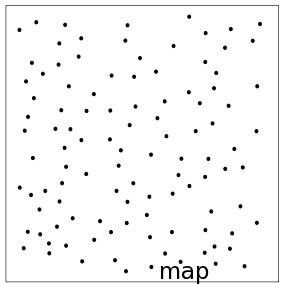
\includegraphics[width=5.8cm]{imgs/region.png}
  \label{fig:region0} 
  }
  \subfigure[2 regions $r_1$ and $r_2$ in time $t_1$ and $t_2$ ]{ % Começa a incluir a figura fig1.pdf
   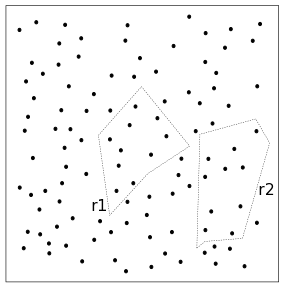
\includegraphics[width=5.8cm]{imgs/region1.png}
  \label{fig:region1} 
  }\\  % Termina de incluir a figura fig1.pdf
  \subfigure[2 regions $r_1$ and $r_2$ with intersection ]{ % Começa a incluir a figura fig2.pdf na mesma linha da figura fig1.pdf
    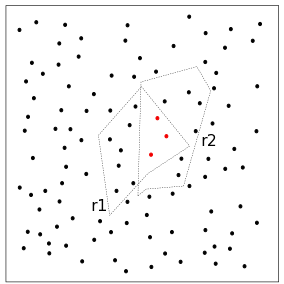
\includegraphics[width=5.8cm]{imgs/region2.png}
   \label{fig:region2}
  } % Termina de incluir a figura fig2.pdf
  % Com esse comando iremos incluir a última figura na próxima linha
  \subfigure[4 regions $r_1$ ... $r_4$ in time $t_1$ and $t_2$ ]{ % Começa a incluir a figura fig3.pdf na linha abaixo
    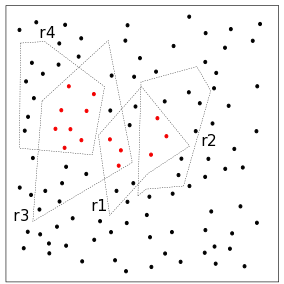
\includegraphics[width=5.8cm]{imgs/region3.png}
     \label{fig:region3} 
  } % Termina de incluir a figura fig3.pdf
 

  \caption{Definition and intersection of regions}
  \label{fig:regions}
\end{figure} % Fecha o ambiente de figuras

The figures in\ref{fig:regions} show an example of regions and their intersections. The points shown in the figure are spatial dataset points (not mouse tracking points), which are highlighted from the regions captured by the mouse tracking. In figure \ref{fig:region0}, it shows the points of the arranged dataset. In figure \ref{fig:region1} it shows 2 regions ($r_1$ and $r_2$) defined from the mouse tracking at a time $t_1$ and $t_2$ where $t_1 \prec t_2$ and that there is no intersection between them. Figure \ref{fig:region2} also shows 2 regions ($r_1$ and $r_2$) defined from mouse tracking at a time $t_1$ and $t_2$ where $t_1 \prec t_2$, and where there is an intersection between them. The intersection between these regions highlights 3 points from the spatial dataset. Figure~\ref{fig:region3} shows 4 regions ($r_1$, $r_2$, $r_3$ and $r_4$) defined from mouse tracking at a time $t_1$ and $t_2$ where $t_1 \prec t_2 $. Regions $r_1$ and $r_4$ were captured at time $t_1$, and regions $r_2$ and $r_3$ at time $t_2$. After capturing the regions, we notice that there are 3 intersections, being the intersections \{$r_1$ and $r_2$\},\{$r_1$ and $r_3$\} and \{$r_3$ and $r_4$\}. For each intersection we have 3, 3 and 8 points highlighted in the dataset, respectively.

%As figuras mostram um exemplo de regioes e suas intersecoes. Os pontos apresentados na figura são pontos do spatial dataset, que são destacados a partir das regiões capturadas a partir do rastreamento no mouse. Na figura X, mostra os pontos do dataset dispostos. Na figura F mostra 2 regioes (r1 e r2) definidas a partir do rastreamento do mouse em um tempo t1 e t2 onde t1 é anterior a t2 e não há  interseção entre elas. A figura F3 mostra 2 regioes (r1 e r2) definidas a partir do rastreamento do mouse em um tempo t1 e t2 onde t1 é anterior a t2, onde há  interseção entre elas. A interseção entre as regiões destacam 3 pontos do dataset. A figura F4 mostra 4 regioes (r1, r2, r3 e r4) definidas a partir do rastreamento do mouse em um tempo t1 e t2 onde t1 é anterior a t2, as regiões r1 e r4 foram definidas no tempo t1, e as regiões r2 e r3 no tempo t2. Após a captura das regiões, notamos que há 3 interseções, sendo elas {r1 e r2}, {r1 e r3} e {r3 e r4}. Para cada interseção temos 3, 3 e 8 pontos do dataset destacados, respectivamente.   



\section{Overlapping Polygons by Clustering Spatiotemporal Data}
\label{sec:overpolygons}

This section presents some definitions and concepts in order to describe (\textit{i}) how the polygons are created,(\textit{ii}) in which delay of time the set of polygons are grouped, (\textit{iii})  why and how the polygons are overlapped and  (\textit{iv}) how the regions of preferences over time are defined.



Figure \ref{fig:paris} presents a sequence of maps of Paris, showing a possible  evolution of how can be captured preference regions from \textit{Ben\'icio} search.

Figure \ref{fig:paris0} shows the map before the to use by  \textit{Ben\'icio}. The Figure \ref{fig:paris1} shows 2 regions where the user searched for locations in a time interval $t_1$ (lets consider $n$ seconds as a time interval, and $n < 60$). These two regions intersect each other. The figure \ref{fig:paris2} presents other 2 regions where apartments were also searched at a time interval $t_2$, where $t_1 \prec t_2$. In the same way, figure \ref{fig:paris3}  presents 2 more regions where apartments were searched in a time interval $t_3$, where $t_1 \prec t_2 \prec t_ 3$.

Figures \ref{fig:paris4} and \ref{fig:paris5} highlight the intercessions of all regions. These intercessions show that these regions have been trafficked by the analyst more than once. It can inform a certain preference in these regions. These regions can be captured from mouse tracking or even by gaze techniques. Recognizing highlighted regions can help the analyst to consider one more parameter in the query to identify points in a particular dataset that may be more in line with their needs.

Considering a preference order of regions for \textit{Ben\'icio}, the possible areas for rent would be: (\textit{i}) the intersection of the regions ($r_1 \cap r_2 \cap r_n$), (\textit{i}) the union of the regions minus their intersections (($r_1 \cup r_2 \cup r_n$) - ($r_1 \cap r_2 \cap r_n$)), and finally (\textit{iii}) the entire dataset.


\begin{figure} % Inicia o ambiente de figuras
\centering
  \subfigure[Paris map.]{ % Começa a incluir a figura fig1.pdf
   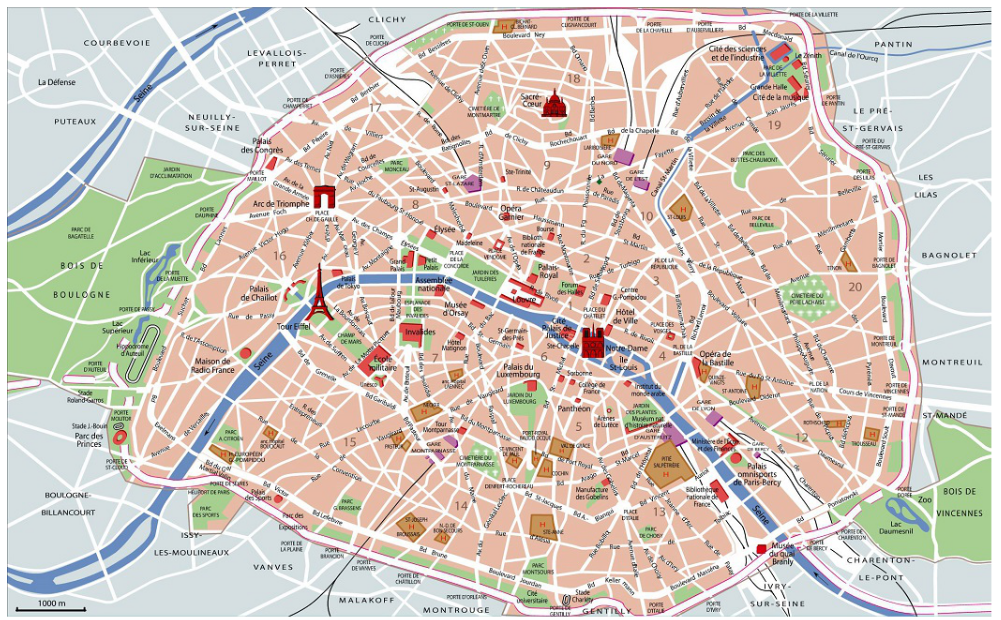
\includegraphics[width=5.8cm]{imgs/adbis2_map0.png}
  \label{fig:paris0} 
  } % Termina de incluir a figura fig1.pdf
  \subfigure[Clusters - time t1.]{ % Começa a incluir a figura fig2.pdf na mesma linha da figura fig1.pdf
    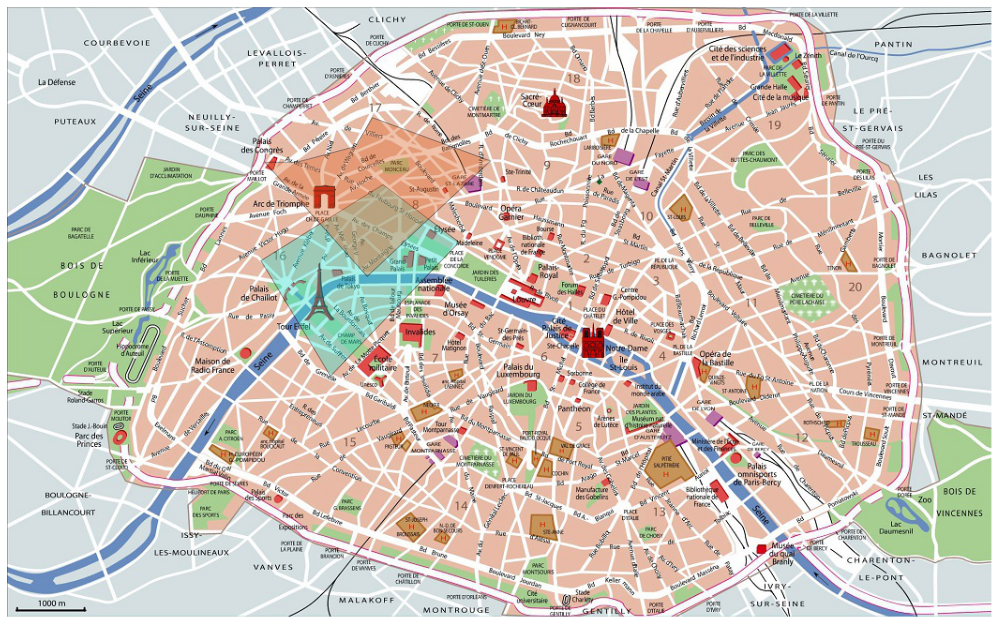
\includegraphics[width=5.8cm]{imgs/adbis2_map1.png}
   \label{fig:paris1}
  } % Termina de incluir a figura fig2.pdf
  \\ % Com esse comando iremos incluir a última figura na próxima linha
  \subfigure[Clusters - time t2.]{ % Começa a incluir a figura fig3.pdf na linha abaixo
    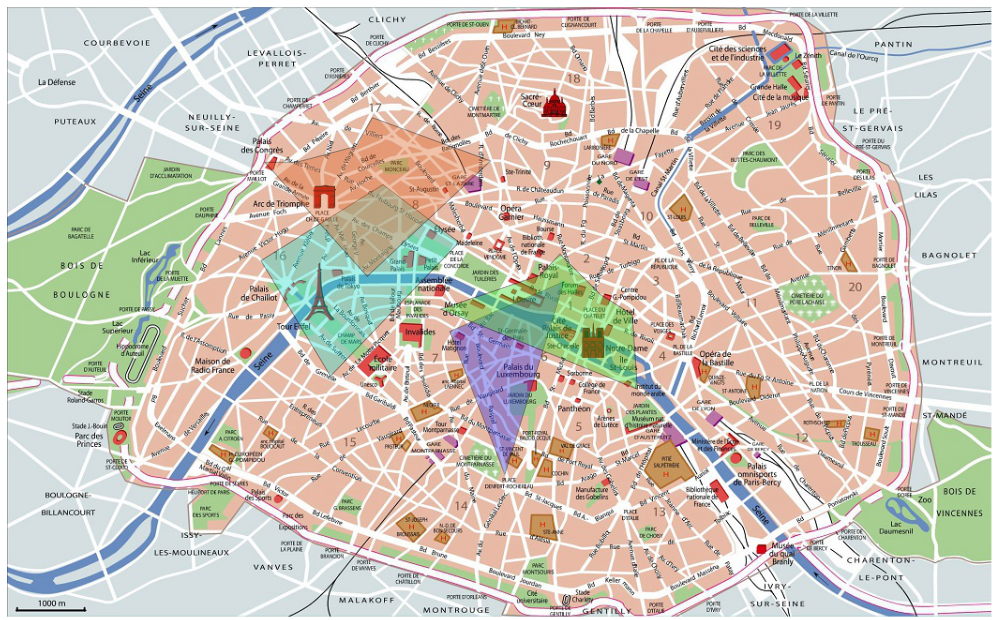
\includegraphics[width=5.8cm]{imgs/adbis2_map2.png}
     \label{fig:paris2} 
  } % Termina de incluir a figura fig3.pdf
   \subfigure[Clusters - time t3.]{ % Começa a incluir a figura fig2.pdf na mesma linha da figura fig1.pdf
    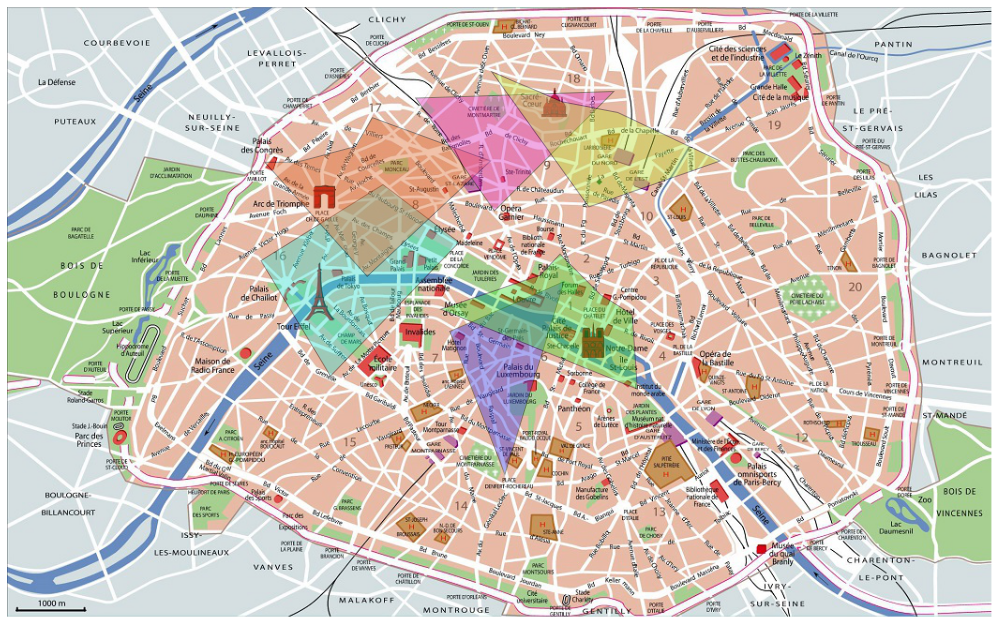
\includegraphics[width=5.8cm]{imgs/adbis2_map3.png}
       \label{fig:paris3} 
  } % Termina de incluir a figura fig2.pdf
  \\ % Com esse comando iremos incluir a última figura na próxima linha
  \subfigure[Intersection of regions.]{ % Começa a incluir a figura fig3.pdf na linha abaixo
    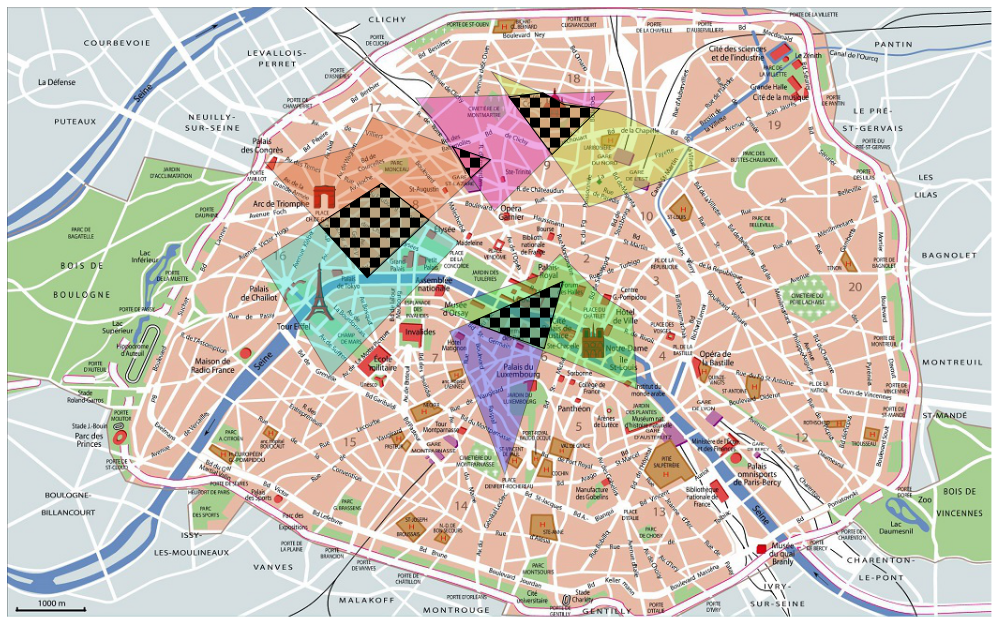
\includegraphics[width=5.8cm]{imgs/adbis2_map4.png}
       \label{fig:paris4} 
  } % Termina de incluir a figura fig3.pdf
   \subfigure[Highlighted regions.]{ % Começa a incluir a figura fig2.pdf na mesma linha da figura fig1.pdf
    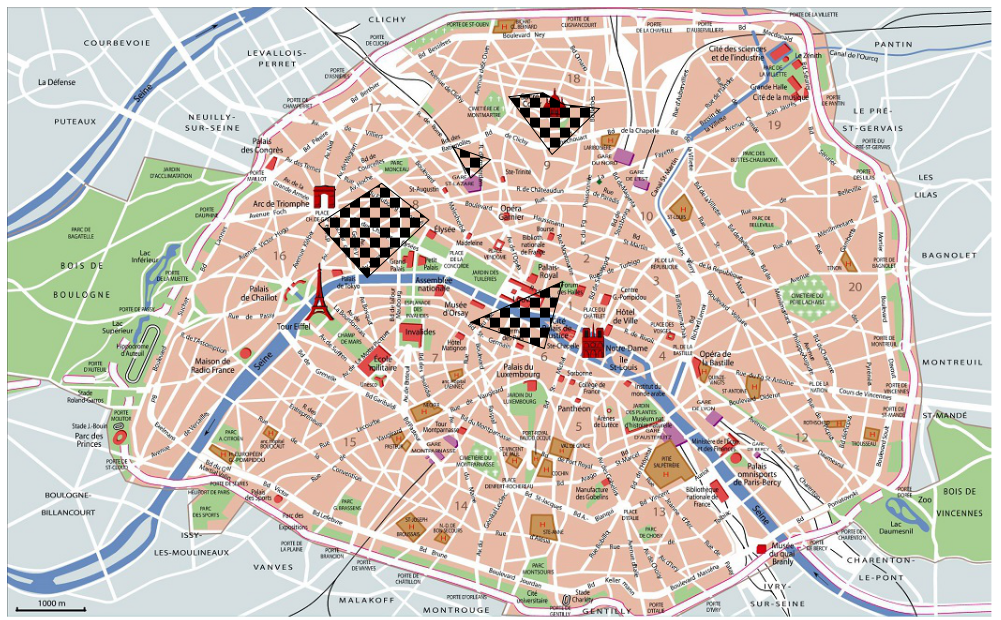
\includegraphics[width=5.8cm]{imgs/adbis2_map5.png}
      \label{fig:paris5} 
  } % Termina de incluir a figura fig2.pdf
  \\ % Com esse comando iremos incluir a última figura na próxima linha
  \caption{Highlighting preference of regions from mouse tracking. }
  \label{fig:paris}
\end{figure} % Fecha o ambiente de figuras


\begin{algorithm}[t]
	\DontPrintSemicolon
	\KwIn{${\cal R}$ = \{ $r_1, r_2,...,r_n $ \}, $\Delta t \in T$}
	% \KwOut{${\cal S}_p$}
	${ R_p} \gets \emptyset$\;\label{cd:definereturn}
	%$p_{next} \gets get\_next(\mathit{{\cal L}^p})$\;\label{cd:getnext}
	\For{$(r_n \in {\cal R})$}{\label{cd:beginfr}
		\For{$(r_{n+1} \in {\cal R})$}{
			\If{$(r_n \cap r_{n+1} \neq \emptyset \wedge get\_time(r_n) \subseteq t \wedge get\_time(r_{n+1}) \subseteq t $}{\label{cd:if_intersectino}
				${ R_p} \gets  (r_n \cap r_{n+1}) \wedge { R_p}  $\;
			}
		}
	}
	%	$p_{next} \gets get\_next({\cal L}_p)$\;}\label{cd:endwhile}
	\Return{${ R_p}$}\; 
	\caption{{\sc Region Highlighter} Algorithm}
	\label{algo:intersectionAlgo}
\end{algorithm}

The Algorithm \ref{algo:intersectionAlgo} goal is to identify which regions are intersect considering the clusters identified during  the analyst search. The inputs are a set o regions ${\cal R}$  and a time interval $\Delta t$. The list of preferred regions is defined in line \ref{cd:definereturn}. For each region $r_n \in {\cal R}$ (line \ref{cd:beginfr}), the algorithm verifies if there are intersections with  a region $r_{n+1} \in {\cal R}$ (line \ref{cd:if_intersectino}). If there is a intersection and the region time is in the time interval, the intersection $r_n \cap r_{n+1} $ is included in ${ R_p}$.

%For instance, on a bike-sharing dataset, ${\cal A}_p = \langle${\tt female}, {\tt young}, {\tt hybrid-bike}$\rangle$ on the schema ${\cal A} = \langle${\tt gender}, {\tt age}, {\tt type}$\rangle$ denotes that $p$ is associated to a young female cyclist who rides a hybrid bike. The set ${\cal A}$ is domain-dependent and defines the semantics of a spatiotemporal dataset.


\begin{algorithm}[t]
	\DontPrintSemicolon
	\KwIn{$p \in {\cal P}$, $\sigma$, $k$, $tlimit$, $R_{p}$ = \{ $r_{p1}, r_{p2},...,r_{pn} $ \}}
	% \KwOut{${\cal S}_p$}
	${\cal S}_p \gets get\_top\_k(\mathit{{\cal L}^p})$\;\label{cd:gettopk}
	$p_{next} \gets get\_next(\mathit{{\cal L}^p})$\;\label{cd:getnext}
   ${\cal S}_{rp} \gets {\cal S}_p$\;\label{cd:empty_regions}
	\While{$(tlimit$ $not$ $exceeded \wedge relevance(p,p_{next}) \geq \sigma)$}{\label{cd:beginwhile}
		\For{$p_{current} \in {\cal S}_p$}{
			\If{$\mathit{diversity\_improved}({\cal S}_p,{\cal S}_{rp},p_{next},p_{current})$}{\label{cd:betterdiv}
			    \For{$r_{current} \in  R_p$}{
			    		   \If{$p_{current} \in r_{current}$}{ \label{cd:point_in_region}
			    		   		${\cal S}_{rp} \gets \mathit{replace}({\cal S}_{rp},p_{next},p_{current})$\;
				$break$\;
			    		   }
			    }
			
				${\cal S}_p \gets \mathit{replace}({\cal S}_p,p_{next},p_{current})$\;
				$break$\;
			}
		}
		$p_{next} \gets get\_next({\cal L}_p)$\;}\label{cd:endwhile}
	\Return{ ${\cal S}_{rp} \cup {\cal S}_p$
	}\; 
	\caption{{\sc GeoGuide} \cite{Omidvar:2017} +  {\sc Region Highlighter} Algorithm}
	\label{algo:geoh}
\end{algorithm}

Algorithm \ref{algo:geoh} modifies the original {\sc Highlighter} proposal presented in GeoGuide \cite{Omidvar:2017} approach .  
The original begins by retrieving the most relevant points to $p$ by simply retrieving the $k$ highest ranking points in ${\cal L}_p$ (line \ref{cd:gettopk}) and function $get\_next({\cal L}_p)$ (Line \ref{cd:getnext}) returns the next point $p_{next}$ in ${\cal L}_p$ in sequential order. Line \ref{cd:empty_regions} initialize the set of points that will be retrieved by the highlighted regions. At the beginning we consider that there is no preferred regions. So, the sets ${\cal S}_{rp}$ and ${\cal S}_{p}$  are the same. Lines \ref{cd:beginwhile} to \ref{cd:endwhile} iterate over the inverted indexes to determine if other points should be considered to increase diversity while staying within the time limit and not violating the relevance threshold with the selected point. %Since points in ${\cal L}_g$ are sorted on decreasing relevance with $p$, the algorithm can safely stop as soon as the relevance condition is violated (or if the time limit is exceeded).

The algorithm then looks for a candidate point $p_{current} \in {\cal S}_p$ to replace in order to increase diversity. If the candidate point is presented in a region $r$ (line \ref{cd:point_in_region}), the point is included in ${\cal S}_{rp}$, considering the boolean function $\mathit{diversity\_improved}()$ (line \ref{cd:betterdiv}). This function checks if by replacing $p_{current}$ by $p_{next}$ in ${\cal S}_p$, the overall diversity of the new ${\cal S}_p$ increases. If the point is not in the preferred region, it is included into ${\cal S}_p$.

\section{Experiments}
\label{sec:experiments}


\section{Conclusion}
\label{sec:conclusions}





\vspace{-5pt}

\bibliographystyle{abbrv}
\bibliography{main}

\end{document}
